\documentclass[conference,10pt]{IEEEtran}
\usepackage[T1]{fontenc}
\usepackage[utf8]{inputenc}
\usepackage{newtxtext,newtxmath}
\usepackage{amsmath}
\usepackage{booktabs}
\usepackage{tabularx}
\usepackage{array}
\usepackage{graphicx}
\usepackage{algorithm}
\usepackage{algpseudocode}
\usepackage{float}
\usepackage[font=footnotesize,labelfont=sf,textfont=sf]{subcaption}
\usepackage{url}
\usepackage{xcolor}
\graphicspath{{figures/}}
\urlstyle{same}
\setlength{\emergencystretch}{1.5em}
\newcolumntype{Y}{>{\raggedright\arraybackslash}X}
\newcommand{\macroF}{macro $F_1$}
\title{Minority-First Incremental Class Learning with Adaptive Neural-Network Growth}
\author{\IEEEauthorblockN{Adriaan den Haan, 27284808}
\IEEEauthorblockA{27284808@sun.ac.za}}
\begin{document}
\maketitle

\begin{abstract}
Class imbalance can make aggregate accuracy obscure poor recognition of infrequent classes. The study asks whether least-to-most-frequent class introduction and optional hidden-layer growth improve class-balanced neural-network prediction. Conventional all-class training was compared with fixed-capacity and adaptive incremental workflows on three data sets. Settings were chosen on validation data before 90 held-out runs with ten matched optimisation seeds per condition. Adaptive growth did not consistently improve macro $F_1$ or minority recall. On Optical Digits, adaptive macro $F_1$ was 0.0102 lower than all-class training. The difference remained statistically significant after correction for six planned tests. The adaptive models contained 27.4--62.8\% fewer parameters but required 3.87--6.48 times as many gradient updates as the all-class models. Adaptive growth therefore reduced final model size without reducing training work. The Optical Digits result therefore argues against a universal predictive benefit under the evaluated design.
\end{abstract}

\section{Introduction}

Imbalanced classification assigns unequal numbers of training observations to target classes. Frequent classes then occur in more minibatch updates, while aggregate accuracy gives greater influence to frequent evaluation classes. The investigation examines whether a minority-first schedule changes class-balanced performance and whether gradual capacity growth provides a smaller useful model.

\subsection{Motivation}

An unweighted objective exposes the optimiser to more examples from frequent classes. Overall accuracy also weights classes according to evaluation frequency. He and Garcia show that class imbalance interacts with class overlap and sample size~\cite{he2009}. Other sources of difficulty also matter. Evaluation must therefore examine individual classes as well as aggregate correctness.

Incremental class learning expands the set of labels available during training. The minority-first version begins with the two least frequent classes and introduces the remaining classes in ascending frequency order. The adaptive workflow also begins with a linear classifier and adds hidden neurons when validation progress stalls while training performance remains below a preset target. The mechanism changes the schedule and optimiser history. Training work also changes, so the experiment compares complete workflows rather than isolating class order.

\subsection{Research Questions and Scope}

Three workflows use the same data partitions. The all-class baseline provides a conventional reference. Fixed incremental training retains a 16-neuron hidden layer, so comparison with adaptive incremental training more directly examines structural growth within the shared schedule. Comparison with all-class training includes the schedule and stage count. Optimiser resets and consolidation also differ. Training work is unequal.

\noindent\textbf{RQ1:} Does minority-first incremental training change test macro $F_1$ relative to all-class training? \textbf{RQ2:} Does the incremental schedule change recognition of predefined minority classes? \textbf{RQ3:} Does adaptive growth reduce final capacity while retaining predictive performance? \textbf{RQ4:} What retention behaviour and training cost accompany the incremental workflows?

The contribution is a reproducible comparison that separates adaptive growth from a fixed incremental control. Predictive and class-specific evidence accompanies structural and computational measurements. The design does not support a causal claim about class order alone because the workflows have unequal update budgets and different optimiser histories.

\section{Background}

The background defines the evaluation objective and neural representation. Incremental learning then motivates the growth and retention diagnostics. The concepts provide the basis for the implemented comparison.

\subsection{Imbalance and Class-Balanced Evaluation}

For a target class, precision measures the fraction of predicted members belonging to the class. Recall measures the fraction of actual members recovered by the classifier. The harmonic mean of precision and recall defines the classwise $F_1$ score. Macro $F_1$ averages the classwise scores without frequency weighting.

Sokolova and Lapalme distinguish how multiclass measures aggregate class-specific errors~\cite{sokolova2009}. That distinction motivates reporting balanced accuracy and macro $F_1$ rather than accuracy alone. Balanced accuracy equals mean class recall in the multiclass setting. Macro $F_1$ also reflects precision, so frequent prediction of a minority label cannot appear favourable through recall alone.

Class frequency does not determine class difficulty. An infrequent class with a distinct feature distribution can remain easy to separate. An abundant class with overlapping features can remain difficult. He and Garcia discussed the interaction between imbalance and other properties of the classification problem~\cite{he2009}. Per-class evidence is necessary to distinguish frequency effects from overlapping decision regions.

\subsection{Neural Capacity and Optimisation}

A feedforward classifier maps numerical features to class scores called logits. Softmax normalisation converts the logits into probabilities that sum to unity. The predicted class receives the largest probability. Cross-entropy penalises low probability assigned to the correct label.

Hidden neurons add nonlinear transformations to the classifier. Insufficient capacity restricts the available decision boundaries. Excess capacity increases the opportunity to fit training-specific variation. Bishop explains how capacity and regularisation affect generalisation~\cite{bishop2006}. The relationship motivates validation-guided stopping and weight decay in the present models.

The rectified linear unit is abbreviated ReLU. The activation returns zero for negative input and preserves non-negative input. The selected network used ReLU hidden activations. Kingma and Ba introduced adaptive moment estimation as an optimiser based on gradient-moment estimates~\cite{kingma2015}. The optimiser is abbreviated Adam. Adam supplied the common optimiser across the three workflows.

\subsection{Incremental Learning and Retention}

Class-incremental learning enlarges the available label set over successive stages. New-class updates can alter parameters that support earlier classes. A later reduction in an earlier class's recall is called forgetting. Parisi \textit{et al.} review the stability problem and rehearsal-based responses in continual neural learning~\cite{parisi2019}.

Full rehearsal keeps every training example from each introduced class in later stages. Earlier classes therefore continue to contribute gradient updates after a new class enters. The present study imposes no memory limit, unlike continual-learning settings that store only a small subset of earlier examples.

Constructive growth starts with a small model and adds capacity during training. Function-preserving transformations have previously been used to widen or deepen networks without immediately changing model outputs~\cite{chen2016}. The additive rule in the present study is a custom implementation. A controller adds one neuron only after stalled validation progress and insufficient training fit. The new neuron contributes zero to every class score at the instant of growth. Later optimisation can make the neuron useful. The safeguard prevents an immediate prediction discontinuity but does not guarantee improved validation performance.

The controller first trains the two least frequent classes. Training and validation behaviour then determine whether the preset conditions request a neuron. The process repeats as classes enter and ends with an all-class consolidation stage. Predictive and retention measurements assess learning behaviour. Final parameters and gradient updates distinguish stored model capacity from training work.

\section{Implementation}

The implementation defines a shared network and three training workflows. A custom controller maps training and validation measurements to explicit stop or growth actions. Saved configurations and checksums make those actions reproducible.

\subsection{Shared Network and Structural Changes}

The model combines a direct linear input-to-output path with one hidden layer. Each hidden neuron adds one nonlinear correction to every class score, and adaptive growth changes only the number of these corrections. Let $d$ denote the feature count and $k$ the current number of output classes. The input vector is $\mathbf{x}\in\mathbb{R}^{d}$ and the hidden-unit count is $h$. The direct-path matrix is $\mathbf{W}\in\mathbb{R}^{k\times d}$ with output-bias vector $\mathbf{b}\in\mathbb{R}^{k}$. Hidden neuron $j$ has input weights $\mathbf{u}_j$ and scalar bias $a_j$. The output weights of neuron $j$ form vector $\mathbf{v}_j$. With activation function $\phi$, the logit vector $\boldsymbol{\ell}$ is
\begin{equation}
\boldsymbol{\ell}=\mathbf{W}\mathbf{x}+\mathbf{b}
 +\sum_{j=1}^{h}\mathbf{v}_j\phi(\mathbf{u}_j^{\mathsf{T}}\mathbf{x}+a_j).
\label{eq:network}
\end{equation}
The direct path supports a linear classifier when $h=0$. Every hidden neuron contributes an additive nonlinear term. The parameter count $m$ is consequently
\begin{equation}
m=(d+1)k+h(d+k+1).
\label{eq:parameters}
\end{equation}
Both fixed-width controls use the same architecture with $h=16$.

A new hidden neuron receives random input weights, but every outgoing weight starts at zero. The new neuron's term in Equation~\ref{eq:network} therefore equals zero for every input. Existing logits and predictions do not change at that instant. Later optimisation can move the outgoing weights away from zero and use the added unit. Output-class expansion is different: existing logit parameters are copied and a new output row is added, but softmax probabilities still change because the new class enters the normalising sum.

\subsection{Adaptive Controller}

Class frequencies in the retained training partition determine the introduction order. Frequency ties use the deterministic encoded-label order. The adaptive network starts with two outputs and no hidden neurons. Each stage rehearses every retained example belonging to the current label set.

The controller uses unsmoothed epoch-end training and validation macro $F_1$. Validation cross-entropy supplies an additional overfitting diagnostic. After nine observations since the last growth event, a plateau compares two historical maxima. The maximum validation score from the latest eight observations must not exceed the earlier maximum by more than 0.001.

At a plateau, underfitting requires training macro $F_1$ below 0.95. The training-minus-validation score gap must also be at most 0.08. Both conditions request an additional neuron when fewer than 16 hidden neurons exist. Otherwise the controller ends the stage.

An overfitting exit requires both a training-minus-validation score gap of at least 0.15 and validation loss more than 0.001 above the lowest earlier loss. The check begins after eight post-growth observations. A hard total budget of 60 epochs overrides other stage decisions.

These constants are pre-test engineering controls rather than theoretically optimal values. Eight epochs provide a short observation window while keeping the staged pilot tractable, and 0.001 defines the same material-improvement tolerance used by static early stopping. The 0.95 training-fit target encodes the intended meaning of insufficient fit. Gaps of 0.08 and 0.15 separate growth from a conservative overfitting exit, but were not estimated from a published rule. The 16-unit cap matches the fixed models' selected width, while the 60-epoch cap bounds each stage. The pilot varied the training-fit target only inside coupled configurations, so causal justification does not follow from that search.

Every strict validation-score improvement updates the best checkpoint. Tied scores retain the earlier checkpoint. Before growth, the network restores the best checkpoint and adds a function-preserving neuron. Adam is rebuilt and the local decision history is cleared. The total stage budget does not reset.

Algorithm~\ref{alg:adaptive} summarises the procedure. The pseudocode gives priority to the hard budget and the overfitting exit. The numerical rules above define the plateau and underfitting decisions precisely.

\begin{algorithm}[t]
\caption{Minority-first adaptive class learning}
\label{alg:adaptive}
\begin{algorithmic}[1]
\Require Training and validation partitions with fixed controls
\State Order classes by increasing training frequency
\State Initialise two outputs and zero hidden neurons
\State Select all retained examples of the introduced classes
\State Train an epoch and evaluate training and validation measures
\State Preserve the highest validation-score checkpoint
\State End the stage when the total budget is exhausted
\State Otherwise end the stage when both overfitting conditions hold
\State Otherwise inspect stagnation after the required observation window
\State At stagnation, restore the best checkpoint
\State Add a hidden neuron when underfitting and spare capacity coincide
\State After growth, rebuild the optimiser and clear local histories
\State End the stage when stagnation does not justify growth
\State Repeat epoch training until the stage ends
\State Restore the best checkpoint and introduce the next class if available
\State Repeat stage training until every class has appeared
\State Consolidate on all training classes and retain the best checkpoint
\State Evaluate the selected model on the held-out test partition
\end{algorithmic}
\end{algorithm}

\subsection{Comparison Methods and Consolidation}

The all-class baseline provides the conventional training reference. The network uses 16 hidden neurons and receives every class immediately. Training ends after eight epochs without a score improvement exceeding 0.001 or after 60 epochs. Every smaller strict score improvement remains eligible for checkpoint selection. The final model restores the highest validation-score checkpoint.

Fixed incremental training uses the same 16-neuron width at every class stage. Class order and rehearsal data match adaptive training. The stage structure also matches, making the comparison more specific to hidden-layer growth. Static validation stopping applies separately to each stage. Output expansion retains earlier parameters but resets Adam.

Both incremental methods receive 15 additional all-class consolidation epochs. Consolidation adds no hidden neurons. The initial consolidation checkpoint competes with all 15 epoch-end checkpoints. The all-class baseline receives no separate consolidation period. The comparison therefore measures different training workflows rather than equal update budgets.

\subsection{Software and Verification}

Python~3.12 and a custom \texttt{torch.nn.Module} implemented the additive network on one processor thread. Custom code implemented the training loops and class schedule. The growth controller and checkpoint restoration were also custom. PyTorch's Adam optimiser minimised an unweighted functional cross-entropy loss. Scikit-learn supplied stratified train/test splitting and the StandardScaler transformer. Scikit-learn also supplied classification metrics but no classifier. The Linux-executable code and analysis scripts are available in the repository.\footnote{Code: \path{github.com/adriaandh1/ml741-assignmen3-27284808}.}

Each run saved dataset hashes and exact source-row split indices. Package versions and hashes identified the executed source files. Checkpoints included the label map and model shape. Regenerated predictions matched every saved final prediction. Independent calculations also reproduced the metrics. Three Dry Bean runs chosen before final score inspection reproduced weights and growth events exactly. The checks establish repeatable execution rather than universal statistical validity.

\section{Empirical Process}

The empirical process separated configuration selection from test assessment. Data audits and preprocessing established the evaluation partitions. A small validation-only pilot then selected shared settings before repeated final training.

\subsection{Data Sets and Audit}

Dry Bean contained 13,611 observations from seven varieties with 16 numerical image-derived features. Koklu and Ozkan introduced the classification problem through measurements of segmented bean images~\cite{koklu2020}. The UCI archive supplied the numerical representation~\cite{ucidrybean}.

Landsat contained 6,435 observations with 36 spectral-neighbourhood features. The UCI source supplies an official split into 4,435 training rows and 2,000 test rows~\cite{ucilandsat}. Six observed labels represented land-cover categories. The absent source label six was not treated as an observed class.

Optical Digits contained 5,620 observations with 64 block-intensity features and ten labels. The official split contained 3,823 training observations and 1,797 test observations. Alpaydin and Kaynak state that 30 writers supplied the training set and a different 13 supplied the test set~\cite{ucioptdigits}.

Dry Bean contained 68 duplicate feature rows with consistent labels. Retaining one representative before partitioning prevented identical copies from being weighted repeatedly or placed across partitions; the rule does not imply that every repeated real observation is invalid. Landsat and Optical Digits contained no exact feature duplicates. No missing or non-finite feature values were found. Identical features with inconsistent labels would have caused rejection rather than silent target resolution.

The sources supplied no usable group identifiers for development partitioning. Exact-duplicate removal therefore controlled duplicate leakage without eliminating unknown acquisition dependence. Landsat included overlapping spatial neighbourhoods. The supplied row order did not permit reconstruction of spatial groups.

\subsection{Partitioning and Preprocessing}

Dry Bean received a stratified 60/20/20 training/validation/test partition after deduplication. The other problems retained their official test sets. Their official training files were split into 75\% training and 25\% validation. Split seed 741 and validation seed 742 fixed the development partitions.

Table~\ref{tab:data} records the retained sample counts. The imbalance ratio denotes the largest divided by the smallest training-class count. Every validation and test class contained at least 20 observations. Dry Bean retained 104 examples in the smallest test class.

\begin{table*}[t]
\caption{Prepared classification data}
\label{tab:data}
\centering
\begin{tabular}{@{}lrrrrrrr@{}}
\toprule
Data set & Features & Classes & Training & Validation & Test & Imbalance & Minimum test class \\
\midrule
Dry Bean & 16 & 7 & 8,125 & 2,709 & 2,709 & 6.80 & 104 \\
Landsat & 36 & 6 & 3,326 & 1,109 & 2,000 & 2.59 & 211 \\
Optical Digits & 64 & 10 & 1,149 & 956 & 1,797 & 10.07 & 174 \\
\bottomrule
\end{tabular}
\end{table*}

Optical Digits was nearly balanced, so training-only downsampling with seed 743 created a controlled long tail for the imbalance question. A geometric schedule gave every successive digit a similar proportional decrease. The extremes retained 282 examples of digit zero and 28 of digit nine, producing a ratio of 10.07 after rounding. Validation and test distributions remained unchanged so evaluation represented the source distributions rather than the imposed training skew. The artificial shift limits direct generalisation to naturally imbalanced digit data.

Standardisation placed features on comparable scales for gradient-based optimisation. Means and standard deviations came only from retained training rows and were then applied unchanged to validation and test data. Downsampling preceded scaler fitting. Three constant Optical Digits training features received unit scale to avoid division by zero. No test information influenced scaling or class order. Natural imbalance was preserved in Dry Bean and Landsat.

\subsection{Pilot Selection and Frozen Controls}

The pilot asked whether activation and learning rate produced stable validation performance across all three workflows. Regularisation and fixed width also varied. Four complete configurations were screened on seed 741 for each data set. Batch size and stopping limits remained fixed, as did most controller rules. The two higher-scoring configurations per data set received confirmation runs on seeds 742 and 743. The complete pilot contained 72 validation-only runs.

Table~\ref{tab:search} presents the coupled settings. Candidate labels identify complete configurations rather than isolated parameter changes. Selection averaged validation macro $F_1$ across methods, preventing one workflow from determining shared controls. Validation-only selection chose the rectified configuration for every data set. Complete candidate results are retained with the experiment artefacts. The selected settings were frozen before any test prediction was computed.

\begin{table*}[t]
\caption{Pilot configurations and shared training controls}
\label{tab:search}
\centering
\begin{tabular}{@{}llrrrr@{}}
\toprule
Candidate & Activation & Learning rate & Weight decay & Fixed width & Training-fit threshold \\
\midrule
Fast hyperbolic & Hyperbolic tangent & 0.010 & 0.0001 & 16 & 0.95 \\
Medium hyperbolic & Hyperbolic tangent & 0.003 & 0.0001 & 16 & 0.95 \\
Rectified & Rectified linear unit & 0.010 & 0.0001 & 16 & 0.95 \\
Small hyperbolic & Hyperbolic tangent & 0.010 & 0.0010 & 8 & 0.90 \\
\bottomrule
\end{tabular}
\end{table*}

The search did not establish global optimality. The small hyperbolic candidate changed width together with regularisation and the training-fit threshold, so the effect of any one change cannot be identified. Batch size 128 and a 16-neuron capacity cap bounded runtime.

Adam used learning rate 0.01 with moment coefficients 0.9 and 0.999. The numerical stabiliser was $10^{-8}$. Coupled weight decay of 0.0001 applied to every trainable parameter. Unweighted cross-entropy supplied the classification objective without oversampling or class weights. Reported predictive cross-entropy excluded the regularisation contribution.

Fixed-method patience was eight epochs with a 60-epoch cap, and incremental consolidation lasted 15 epochs. Final seeds 1001 through 1010 yielded 90 runs across the three methods and three data sets.

A separate one-factor sensitivity check addressed the arbitrary controller constants without revising the locked experiment. Only adaptive models were retrained on the existing validation partitions with pilot seeds 741--743. The training-fit threshold produced substantial structural changes, as Table~\ref{tab:sensitivity} shows. A threshold of 0.90 suppressed Dry Bean growth, while 0.98 reached the 16-unit cap in every seed. Validation scores changed less than model size. The controller therefore cannot be described as selecting a unique architecture independently of the preset target. Repository artefacts retain changes to the plateau rule and overfitting gap. Growth-cap and epoch-cap variants are also retained.

\begin{table}[t]
\caption{Validation sensitivity to training-fit target}
\label{tab:sensitivity}
\centering
\begin{tabular}{@{}lccc@{}}
\toprule
Data set & 0.90 & 0.95 & 0.98 \\
\midrule
Dry Bean & 0.9425 / 0.0 & 0.9473 / 3.3 & 0.9488 / 16.0 \\
Landsat & 0.8514 / 5.7 & 0.8598 / 10.3 & 0.8578 / 12.3 \\
Optical Digits & 0.9410 / 0.0 & 0.9405 / 0.3 & 0.9414 / 1.0 \\
\bottomrule
\end{tabular}
\par\vspace{4pt}
\begin{minipage}{0.98\columnwidth}\footnotesize Entries are mean validation macro $F_1$ / final hidden units across three pilot seeds.\end{minipage}
\end{table}

\subsection{Measures and Paired Uncertainty}

Macro $F_1$ supplied the primary measure because every class receives equal weight in the reported average. Precision also prevents high minority recall achieved by excessive minority predictions from appearing favourable by itself. Let $c$ identify a target class and $q$ denote the final class count. Class precision is $p_c$ and recall is $r_c$. The class $F_1$ score $f_c$ and macro score $f_{\mathrm{m}}$ are
\begin{equation}
f_c=\frac{2p_c r_c}{p_c+r_c},\qquad
f_{\mathrm{m}}=\frac{1}{q}\sum_{c=1}^{q}f_c.
\label{eq:metrics}
\end{equation}
A zero precision-plus-recall denominator received a zero score. Accuracy and balanced accuracy supplied complementary summaries. Per-class precision and recall exposed class-specific trade-offs. Test cross-entropy measured the mean negative log-probability assigned to the correct label.

Minority recall averaged the least frequent $\lceil q/3\rceil$ training classes, while majority recall averaged the most frequent $\lceil q/3\rceil$ classes. Thirds provide compact summaries of the two frequency extremes. Middle-frequency classes are excluded to keep those contrasts distinct. The groups were defined from training frequencies before final evaluation and remained fixed across methods and seeds. The descriptive grouping is not a standard imbalance metric, so per-class recall supplements every group comparison. Stage-end validation recall measured retention of previously introduced labels.

Forgetting averaged the non-negative loss from each class-specific best earlier recall to final validation recall. Classes without an earlier observation were excluded. The all-class baseline had no comparable introduction sequence. Baseline forgetting was therefore treated as not applicable.

Within each run, an optimisation seed fixes initial weights and epoch-level minibatch shuffles. The seed also initialises later hidden and output parameters. The workflows consume randomness differently because their architectures and stage trajectories differ, so equal seed numbers do not imply identical random-number sequences. Means and sample standard deviations summarised ten final seeds per condition. Methods were paired by optimisation seed so corresponding stochastic repetitions could be compared under the same fixed data partition.

The basic bootstrap observation was one paired seed. Each of 10,000 bootstrap samples drew ten seed indices with replacement using analysis seed 2741. The same indices selected both methods before the mean paired difference was recomputed. The 2.5 and 97.5 percentiles formed the reported interval. Efron and Tibshirani provide the empirical-resampling framework used here~\cite{efron1993}. The intervals describe optimisation-seed variability under one fixed partition.

The exact sign-flip null treats the positive and negative signs of paired differences as exchangeable. Ten pairs permit all $2^{10}=1,024$ sign assignments to be enumerated for a two-sided test. Holm's sequential procedure controlled the familywise error rate across the six planned incremental-versus-baseline tests~\cite{holm1979}. A statistically significant result means rejection after that correction at the predeclared 0.05 threshold; the term does not imply a large practical effect. Adaptive-versus-fixed comparisons remained descriptive, and the test requires sign symmetry under the null.

The repetitions used fixed data partitions rather than repeated sampling of new data. No interval represented independent geographic generalisation or population-sampling uncertainty. All methods within a data set used the same examples, but the design did not match total computational work.

\subsection{Analysis Procedure}

RQ1 is answered by test macro $F_1$ and seed-level spread. Paired differences and corrected tests determine whether mean ordering has inferential support. A higher observed mean alone is insufficient when the paired interval includes zero or the planned test does not reject. For RQ2, fixed incremental versus all-class training provides the primary schedule comparison; adaptive results additionally include structural growth. The comparison remains between complete workflows rather than isolating class order because update budgets and stage counts differ. Optimiser histories and consolidation also differ. RQ2 uses the predefined minority-group recall first. Per-class recall then reveals effects hidden by the group average. Consistent improvement in minority recall without a material majority reduction would support a favourable minority effect.

RQ3 compares final hidden counts and parameter counts with predictive results. Fewer parameters indicate lower storage and inference capacity, but do not establish equivalent prediction or cheaper training. RQ4 examines stage-end recall and the forgetting diagnostic for retention, then compares gradient updates and runtime for training cost. Earlier-class recall that later declines indicates retention loss, while the absence of a no-rehearsal control prevents attributing a saved amount to rehearsal. Evidence is interpreted across all three data sets; one favourable data set cannot establish a general benefit.

\section{Results and Discussion}

The results compare held-out prediction before examining minority recognition and adaptive behaviour. Computational measurements then establish the cost of reduced capacity. The final discussion separates supported conclusions from limitations.

\subsection{Held-Out Predictive Performance}

Table~\ref{tab:performance} reports the final test results. Macro $F_1$ entries give means and sample standard deviations across ten seeds. Other entries give means. Pilot validation scores were not reused as held-out estimates.

\begin{table*}[t]
\caption{Held-out classification performance}
\label{tab:performance}
\centering
\begin{tabular}{@{}llcccc@{}}
\toprule
Data set & Method & Macro $F_1$ & Accuracy & Balanced accuracy & Cross-entropy \\
\midrule
Dry Bean & All-class & $0.9372\pm0.0022$ & 0.9259 & 0.9372 & 0.2047 \\
 & Fixed incremental & $0.9375\pm0.0022$ & 0.9259 & 0.9385 & 0.2031 \\
 & Adaptive & $0.9365\pm0.0019$ & 0.9254 & 0.9373 & 0.2164 \\
\addlinespace
Landsat & All-class & $0.8655\pm0.0097$ & 0.8821 & 0.8646 & 0.3099 \\
 & Fixed incremental & $0.8725\pm0.0051$ & 0.8866 & 0.8728 & 0.2957 \\
 & Adaptive & $0.8700\pm0.0031$ & 0.8854 & 0.8691 & 0.3041 \\
\addlinespace
Optical Digits & All-class & $0.9210\pm0.0047$ & 0.9222 & 0.9214 & 0.2819 \\
 & Fixed incremental & $0.9207\pm0.0056$ & 0.9219 & 0.9212 & 0.3310 \\
 & Adaptive & $0.9108\pm0.0040$ & 0.9122 & 0.9114 & 0.3156 \\
\bottomrule
\end{tabular}
\end{table*}

Dry Bean produced closely grouped scores. Fixed incremental training exceeded the all-class mean by only 0.0003. Adaptive training fell below the baseline by 0.0007. The differences did not establish a useful predictive advantage from minority-first growth.

The Landsat fixed incremental mean was 0.0070 higher than the all-class mean. The adaptive mean was 0.0045 higher than all-class training and 0.0025 lower than fixed incremental training. Baseline variability exceeded the variability of either incremental method.

Figure~\ref{fig:seed} shows individual seeds for Dry Bean and Landsat. Horizontal marks indicate means rather than confidence bounds. The Landsat baseline included a substantially lower run near 0.841. The paired analysis retained the low run without replacement.

\begin{figure*}[t]
\centering
\begin{subfigure}[t]{3.48in}
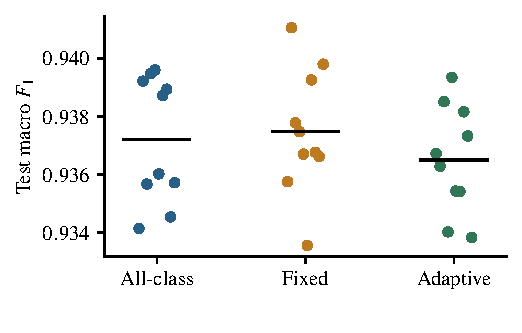
\includegraphics[width=\linewidth]{performance_dry_bean.pdf}
\caption{Dry Bean}
\end{subfigure}\hfill
\begin{subfigure}[t]{3.48in}
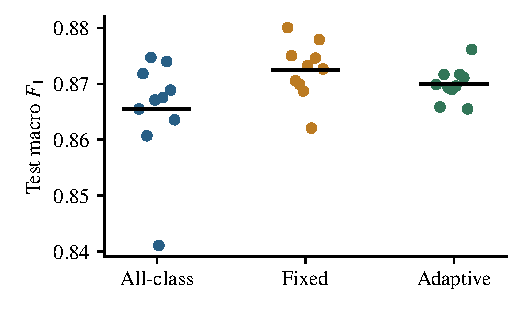
\includegraphics[width=\linewidth]{performance_landsat.pdf}
\caption{Landsat}
\end{subfigure}
\caption{Seed-level test performance. Dots are ten final optimisation seeds; horizontal marks are arithmetic means.}
\label{fig:seed}
\end{figure*}

Optical Digits showed a different pattern. Adaptive training achieved 0.9108 compared with 0.9210 for all-class training. Fixed incremental training remained close to the baseline. The result contradicted a general claim that minority-first exposure necessarily improved final class-balanced recognition.

Cross-entropy supplied additional evidence beyond class predictions. Fixed incremental training on Optical Digits produced similar macro $F_1$ to baseline but larger cross-entropy. The increase from 0.2819 to 0.3310 indicated a less favourable distribution of correct-label probabilities. A similar classification score did not imply a similar probabilistic loss.

\subsection{Paired Differences and Uncertainty}

Table~\ref{tab:paired} gives incremental-minus-baseline differences. Negative values favour the all-class baseline. The intervals are unadjusted paired-bootstrap intervals. The final column gives Holm-adjusted test probabilities for the six-comparison family.

\begin{table*}[t]
\caption{Paired differences from all-class training}
\label{tab:paired}
\centering
\begin{tabular}{@{}llrrrr@{}}
\toprule
Data set & Incremental method & Mean difference & Lower bound & Upper bound & Adjusted probability \\
\midrule
Dry Bean & Fixed & 0.0003 & $-0.0012$ & 0.0017 & 1.0000 \\
 & Adaptive & $-0.0007$ & $-0.0023$ & 0.0009 & 1.0000 \\
Landsat & Fixed & 0.0070 & 0.0011 & 0.0142 & 0.2637 \\
 & Adaptive & 0.0045 & $-0.0010$ & 0.0115 & 0.8906 \\
Optical Digits & Fixed & $-0.0003$ & $-0.0047$ & 0.0039 & 1.0000 \\
 & Adaptive & $-0.0102$ & $-0.0135$ & $-0.0068$ & 0.0117 \\
\bottomrule
\end{tabular}
\end{table*}

Both Dry Bean intervals included zero. The Landsat fixed incremental interval excluded zero before multiplicity correction. The corresponding adjusted probability was 0.2637. The positive unadjusted interval and nonsignificant adjusted test addressed different inferential criteria. Neither finding justified omitting the correction.

The Optical Digits adaptive reduction survived the declared correction. Figure~\ref{fig:paired-digits} expresses the paired differences in percentage points. Adaptive training was approximately 1.02 points lower than baseline. Fixed incremental training showed no comparable directional separation.

\begin{figure}[t]
\centering
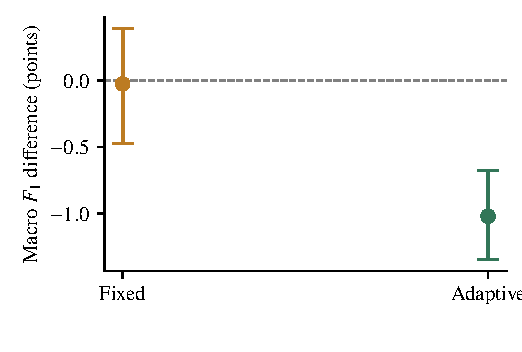
\includegraphics[width=3.48in]{paired_optdigits.pdf}
\caption{Incremental-minus-all-class mean test macro $F_1$ differences in percentage points on Optical Digits. Error bars are unadjusted 95\% paired-bootstrap intervals.}
\label{fig:paired-digits}
\end{figure}

Adaptive capacity did not produce a higher observed mean than fixed incremental capacity on any problem. The descriptive comparison isolates growth more directly than comparison with all-class training but was not part of the six-test inferential family.

\subsection{Minority and Class-Specific Recognition}

Table~\ref{tab:groups} reports the predefined minority and majority groups. Dry Bean minority recall changed little under adaptive training. Landsat showed the clearest descriptive minority improvement. Optical Digits instead showed reductions under both incremental methods.

\begin{table}[t]
\caption{Mean recall by training-frequency group}
\label{tab:groups}
\centering
\begin{tabular}{@{}llrr@{}}
\toprule
Data set & Method & Minority & Majority \\
\midrule
Dry Bean & All-class & 0.9554 & 0.9146 \\
 & Fixed & 0.9578 & 0.9147 \\
 & Adaptive & 0.9556 & 0.9147 \\
Landsat & All-class & 0.7356 & 0.9131 \\
 & Fixed & 0.7648 & 0.9084 \\
 & Adaptive & 0.7478 & 0.9124 \\
Optical Digits & All-class & 0.8511 & 0.9627 \\
 & Fixed & 0.8472 & 0.9661 \\
 & Adaptive & 0.8301 & 0.9589 \\
\bottomrule
\end{tabular}
\end{table}

Landsat fixed incremental training increased minority recall by approximately 2.92 percentage points, while majority recall decreased by approximately 0.47 points. Adaptive training increased minority recall by approximately 1.22 points with a smaller majority decrease. The group summary therefore shows a minority--majority trade-off rather than a uniform change.

Figure~\ref{fig:recall} presents mean per-class test recall. The Dry Bean BOMBAY class was the rarest training class but achieved perfect mean recall under every method. The more frequent SIRA class remained substantially harder. The pattern supports the background argument that imbalance alone does not determine difficulty; overlap and separability also matter.

\begin{figure*}[t]
\centering
\begin{subfigure}[t]{\textwidth}
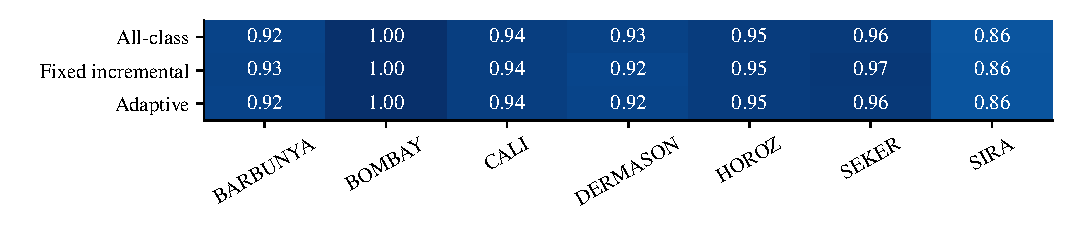
\includegraphics[width=\linewidth]{recall_dry_bean.pdf}
\caption{Dry Bean}
\end{subfigure}
\begin{subfigure}[t]{\textwidth}
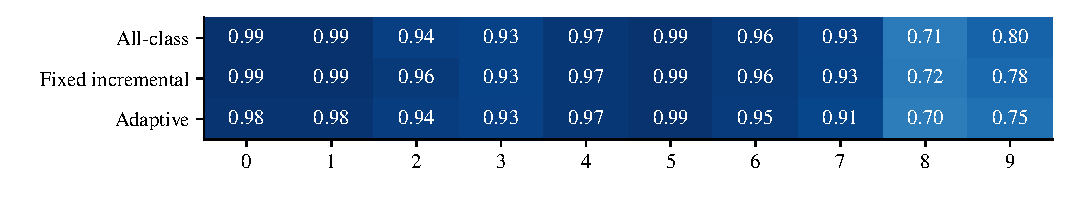
\includegraphics[width=\linewidth]{recall_optdigits.pdf}
\caption{Optical Digits}
\end{subfigure}
\caption{Mean class-specific test recall across ten final seeds}
\label{fig:recall}
\end{figure*}

Optical Digits minority recall fell from 0.8511 to 0.8301 under adaptive training. Digit nine entered in the first stage, yet adaptive mean recall was 0.0483 below baseline and every paired seed showed a reduction. Minority-first exposure therefore did not guarantee better final recognition after all classes entered.

The all-class test recall for digit eight was approximately 0.71, while adaptive recall remained near 0.70. Full rehearsal did not eliminate the difficulty. Adaptive models also averaged only 0.5 hidden units, indicating that the training-fit rule often accepted a nearly linear model even though the separate test writers remained difficult.

\subsection{Capacity Growth and Retention}

Figure~\ref{fig:capacity} shows mean adaptive capacity after each class stage. Landsat requested substantially more growth than Dry Bean. Optical Digits usually retained a linear or nearly linear model.

\begin{figure}[t]
\centering
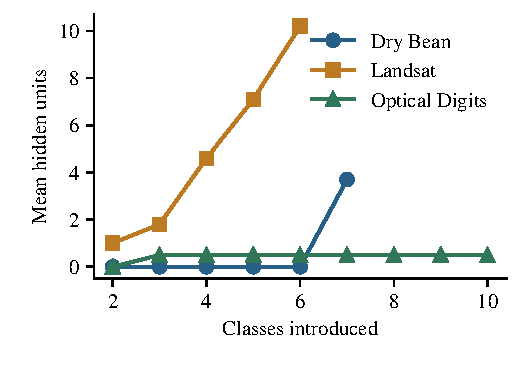
\includegraphics[width=\linewidth]{capacity.pdf}
\caption{Adaptive hidden-layer size after each class stage, averaged across ten final seeds.}
\label{fig:capacity}
\end{figure}

Figure~\ref{fig:retention} shows mean stage-end validation recall for rare digits eight and nine. The final plotted stage denotes consolidation after all ten classes had appeared.

\begin{figure}[t]
\centering
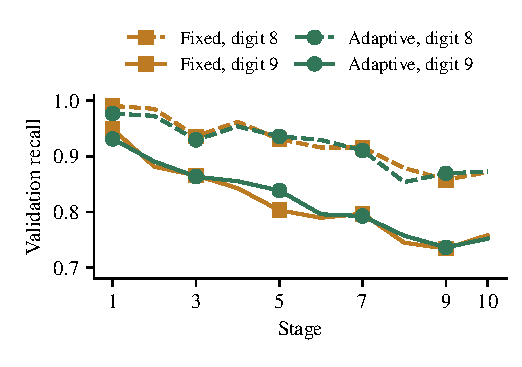
\includegraphics[width=\linewidth]{retention.pdf}
\caption{Rare-digit stage-end validation recall, averaged across ten final seeds. The final stage is consolidation.}
\label{fig:retention}
\end{figure}

The mean final hidden counts were 3.7 for Dry Bean and 10.2 for Landsat. Optical Digits averaged 0.5 hidden units. The sensitivity check shows that such architecture sizes depend on the chosen training-fit target. Meeting that target did not establish adequate capacity for the separate test writers.

The hard epoch cap remained an active constraint. All ten Dry Bean final adaptive class stages reached the 60-epoch limit. Landsat reached the limit in 32 of 50 adaptive class stages. No run exceeded the 16-neuron capacity cap. The results therefore described budget-constrained growth rather than fully converged architecture selection.

Both incremental methods lost recall for digit nine across earlier stages. Consolidation produced partial recovery without restoring the initial level.

Full rehearsal did not eliminate endpoint forgetting. The histories did not measure the immediate before-and-after effect of each introduction. The comparison also lacked a no-rehearsal control. A causal claim that rehearsal prevented a particular amount of forgetting was therefore unsupported.

\subsection{Computational Cost and Practical Interpretation}

Table~\ref{tab:cost} reports model size and training work. Parameters and updates are means across seeds. Runtime includes training and final evaluation but excludes artefact storage. A single processor thread supported sequential execution.

\begin{table*}[t]
\caption{Model capacity and computational cost}
\label{tab:cost}
\centering
\begin{tabular}{@{}llrrrr@{}}
\toprule
Data set & Method & Hidden units & Parameters & Gradient updates & Runtime in seconds \\
\midrule
Dry Bean & All-class & 16.0 & 503.0 & 1,152.0 & 2.15 \\
 & Fixed incremental & 16.0 & 503.0 & 4,207.8 & 7.97 \\
 & Adaptive & 3.7 & 207.8 & 7,467.5 & 5.27 \\
Landsat & All-class & 16.0 & 910.0 & 806.0 & 1.57 \\
 & Fixed incremental & 16.0 & 910.0 & 1,907.4 & 3.96 \\
 & Adaptive & 10.2 & 660.6 & 4,591.2 & 5.74 \\
Optical Digits & All-class & 16.0 & 1,850.0 & 277.2 & 0.64 \\
 & Fixed incremental & 16.0 & 1,850.0 & 922.3 & 2.66 \\
 & Adaptive & 0.5 & 687.5 & 1,072.4 & 1.63 \\
\bottomrule
\end{tabular}
\end{table*}

Adaptive networks reduced parameter counts by 58.7\% on Dry Bean and 27.4\% on Landsat. The reduction reached 62.8\% on Optical Digits. Fewer parameters reduce stored model size and the arithmetic required for one prediction. Dry Bean combined that reduction with a small observed score difference, although no formal equivalence test was performed.

The smaller models required more training work. Adaptive update counts were approximately 6.48 times baseline on Dry Bean and 5.70 times baseline on Landsat. Optical Digits required approximately 3.87 times the baseline updates. Adaptive runtime also exceeded baseline runtime on every problem.

Parameter count did not determine runtime alone. Adaptive Dry Bean used more updates than fixed incremental training but ran faster with smaller intermediate networks. Stage sizes and validation evaluations also affected time. Update counts are less hardware-dependent than wall-clock measurements, but still omit differences in work per update.

All-class training required the least work under the measured setup. Adaptive growth offered smaller stored models without a consistent predictive benefit. Fixed incremental training had the highest observed Landsat mean but required additional computation. No method was preferable on every predictive and computational criterion.

\subsection{Limitations}

The experiment used a fixed partition for each problem. Ten optimisation seeds did not represent ten independently sampled data sets. Seed-bootstrap intervals omitted partition uncertainty and population variation. The sign-flip assumptions further restricted inferential interpretation.

The pilot searched a small set of coupled configurations. A shared selection objective avoided preferential tuning of adaptive training but did not optimise every method independently. The fixed width search covered eight and 16 neurons. No claim of global hidden-width optimality followed from that search.

Training budgets differed across workflows. Full rehearsal and additional class stages increased exposure to earlier classes. Optimiser resets also accompanied structural changes. The comparison did not isolate class order from update count or optimiser-state effects.

Landsat spatial dependence restricted geographic generalisation. Unknown acquisition groups remained possible in Dry Bean. Optical Digits used distinct official test writers but lacked writer-grouped validation identifiers. Training-only downsampling created a deliberately artificial class-frequency shift.

The controller sensitivity check further showed that final width depends on the preset training-fit target. Adaptive performance did not consistently improve minority recognition or macro $F_1$. Endpoint histories showed retention losses without isolating immediate forgetting or rehearsal effects. These limitations qualify the reported capacity--cost trade-off.

\section{Conclusion}

The study investigated whether minority-first incremental training and validation-triggered growth improve imbalanced multiclass learning. Three workflows were compared on fixed partitions after validation-only selection. Paired optimisation seeds quantified training variability conditional on fixed data partitions.

For RQ1, incremental training did not consistently improve macro $F_1$; the corrected Optical Digits result provided evidence against a universal adaptive benefit. For RQ2, minority recall increased descriptively on Landsat but decreased on Optical Digits. Early exposure therefore did not guarantee better final recognition. For RQ3, adaptive growth produced 27.4--62.8\% fewer parameters. The validation sensitivity check showed that final width depends on the training-fit target.

For RQ4, earlier-class recall declined even with full rehearsal. The design cannot quantify how much rehearsal prevented. Smaller adaptive models also required more gradient updates and longer runtime than all-class training. Adaptive growth thus reduced final model size rather than training cost. The next experiments should vary data partitions independently and match update budgets. Class order and rehearsal should then be ablated while the remaining workflow stays fixed.

\clearpage
\IEEEtriggeratref{7}
\begin{thebibliography}{12}
\bibitem{bishop2006}
C. M. Bishop, \emph{Pattern Recognition and Machine Learning}. New York, NY, USA: Springer, 2006.
\bibitem{chen2016}
T. Chen, I. Goodfellow, and J. Shlens, ``Net2Net: Accelerating learning via knowledge transfer,'' in \emph{Proc. 4th Int. Conf. Learning Representations}, San Juan, Puerto Rico, 2016.
\bibitem{efron1993}
B. Efron and R. J. Tibshirani, \emph{An Introduction to the Bootstrap}. New York, NY, USA: Chapman and Hall, 1993.
\bibitem{he2009}
H. He and E. A. Garcia, ``Learning from imbalanced data,'' \emph{IEEE Transactions on Knowledge and Data Engineering}, vol. 21, no. 9, pp. 1263--1284, 2009, doi: 10.1109/TKDE.2008.239.
\bibitem{holm1979}
S. Holm, ``A simple sequentially rejective multiple test procedure,'' \emph{Scandinavian Journal of Statistics}, vol. 6, no. 2, pp. 65--70, 1979.
\bibitem{kingma2015}
D. P. Kingma and J. Ba, ``Adam: A method for stochastic optimization,'' in \emph{Proceedings of the Third International Conference on Learning Representations}, San Diego, CA, USA, 2015.
\bibitem{koklu2020}
M. Koklu and I. A. Ozkan, ``Multiclass classification of dry beans using computer vision and machine learning techniques,'' \emph{Computers and Electronics in Agriculture}, vol. 174, article 105507, 2020, doi: 10.1016/j.compag.2020.105507.
\bibitem{parisi2019}
G. I. Parisi, R. Kemker, J. L. Part, C. Kanan, and S. Wermter, ``Continual lifelong learning with neural networks: A review,'' \emph{Neural Networks}, vol. 113, pp. 54--71, 2019, doi: 10.1016/j.neunet.2019.01.012.
\bibitem{sokolova2009}
M. Sokolova and G. Lapalme, ``A systematic analysis of performance measures for classification tasks,'' \emph{Information Processing and Management}, vol. 45, no. 4, pp. 427--437, 2009, doi: 10.1016/j.ipm.2009.03.002.
\bibitem{ucidrybean}
UCI Machine Learning Repository, ``Dry Bean,'' data set, 2020, doi: 10.24432/C50S4B.
\bibitem{ucilandsat}
A. Srinivasan, ``Statlog (Landsat Satellite),'' UCI Machine Learning Repository, data set, 1993, doi: 10.24432/C55887.
\bibitem{ucioptdigits}
E. Alpaydin and C. Kaynak, ``Optical Recognition of Handwritten Digits,'' UCI Machine Learning Repository, data set, 1998, doi: 10.24432/C50P49.
\end{thebibliography}
\end{document}
